\section{Tilstandsovergangsbetingelsar}
\thispagestyle{fancy}

For at tilstandsmaskina skal få lov til å bytte tilstand er det nokre spesefikke betingelsar som må være oppfylt.
Fleire av betingelsane er styrt av tid og alle desse tidene er justerbare via parameter. \newline
I programmet er betingelsane styrt med IF setningar, men betingelsane er best presentert grafisk.
Vi har laga eit skjema som dokumenterer alle overgangsbetingelsane i tilstandsmaskina. \newline \newline

\begin{figure}[htbp]
    \centering
    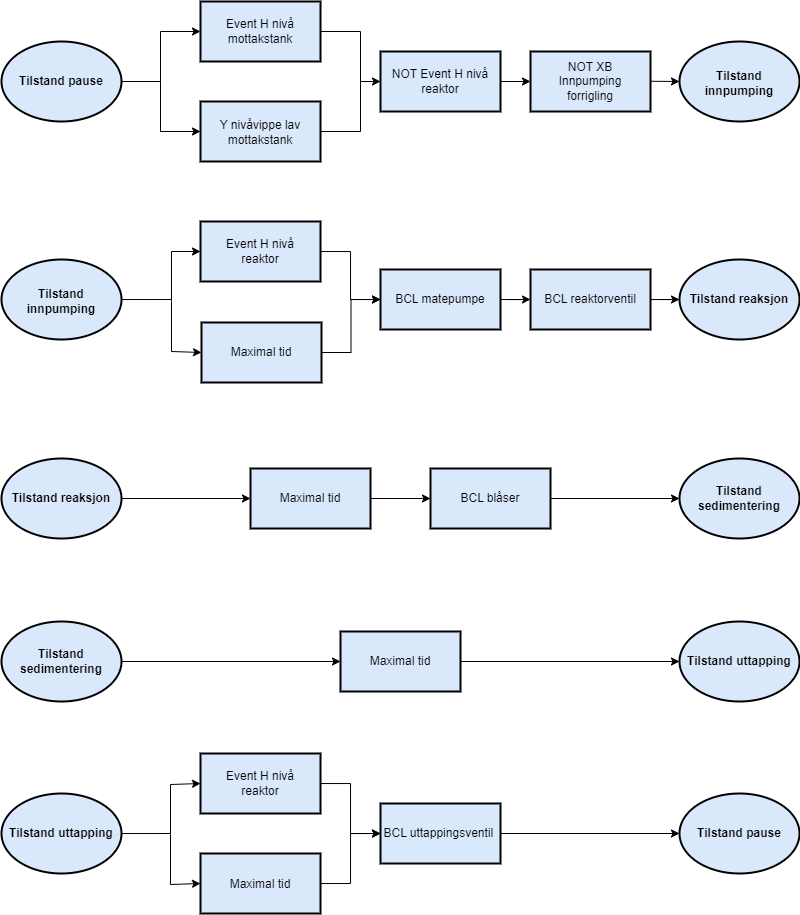
\includegraphics[scale=0.5]{Figurar/Tilstandsovergang.drawio.png}
    \caption{Grafisk representasjon av overgangsbetingelsar}\label{fig:Tilstandsovergangsbetingelsar}
\end{figure}

\newpage